\chapter{Methods}

In this chapter we will concentrate on the main theoretical bases needed for
the computation of physical chemistry methods used on this work. Starting with
the Variational Principle and ending with \gls{ELF} and IQA, going through
\gls{DFT} and Hartree-Fock.

Also, with this chapter we purport to have a general idea about the theory and
postulates taken into account for the results and conclusions in this thesis.
Additionally, we will also give details of computational details.

\section{Quantum Mechanics Foundations}

\begin{flushright}
  {\small
  ``{\em I think I can safely say that nobody
  understands quantum mechanics}''.
  
  -Richard Feynman
  }
\end{flushright}

\normalsize One of the cornerstones of the current physics and one of the
biggest (maybe the biggest until now) paradigm shift for science is Quantum
Mechanics.  Some sources say that William Thomson, 1st Baron Kelvin, never said
``There is nothing new to be discovered in physics now. All that remains is
more and more precise measurement'', and that is just a misattributed quote.
Whether that quote was said by Kelvin or not, fortunately the point of the
quote is not true.

Now we know that even the most powerful mathematical model of universe that we
have, the Standard Model of Particle Physics, cannot predict all the phenomena
that mankind has measured.  And paradoxically, for people outside of science,
the things we cannot predict are what is really interesting for science.

The scientific community thought that Newton made a mistake in describing light
as a particle, since Young's interference experiment showed the wave nature of
light. However, Einstein came with Plank's ideas \cite{Einstein1905} to say
that they both had the correct answer at the same time. Nowadays we know that
is not exactly a duality between waves and particles, but that idea is really
helpful since our brains cannot understand quantum events at all, we can only
imagine them with classic mechanics.

One of the first steps of Quantum Mechanics (as a new theory with its own
mathematical model) was the Schrödinger Equation (Equation \ref{sch_eq}),
postulated by Erwin Schrödinger in 1925, and published one year
after~\citet{Schrdinger1926}. It was reformulated two years after by Dirac for
massive particles with $\sfrac{1}{2}$ spin, taking into consideration
relativistic effects (Equation \ref{dirac_eq})~\citep{Dirac1928}, being one of
the scant bridges between Quantum Physics and Relativity~\cite{Halzen1984}.

\begin{equation}
  \gls{iunit}\gls{hbar}\frac{\partial}{\partial t}\ket{\gls{Psi}} = \left [ \frac{-\hbar^2}{2m}\gls{nablacuadrada}
  + V(\mathbf{r},t) \right ] \gls{Psiket} = \gls{hamiltoniano}\ket{\Psi}
  \label{sch_eq}
\end{equation}

\begin{align}
  i\hbar\gamma^{\mu}\partial_{\mu}\psi - mc\psi = 0
  \label{dirac_eq}
\end{align}

Where $i$ = $\sqrt{-1}$, $\hbar$ is the reduced Plank's constant,
$\gamma^{\mu}$ is the $\mu^{th}$ gamma matrix, and $\partial_{\mu}$ is the
derivative over time and space as $\left( c^{-1}\frac{\partial}{\partial t},
\vec{\nabla} \right)$.

Another bridge between Quantum Physics and Relativity was given by Stephen
Hawking~\cite{HAWKING1974}, with his work about the radiation that occurs at
the event horizon of black holes. This is because this phenomena involves the
Heisenberg's uncertainty principle with the space-time singularities. 

Since the mathematical formulation about the Hawking radiation other
mathematical expressions have been developed, but it was the first expression
with constants from Quantum and Relativity, equation expressed as:

\begin{align}
  T_{H} = \frac{\hbar \gls{cspeed}^{3}}{8\gls{pi} \gls{gconstant}M \gls{kb}}
\end{align}

Nevertheless, in Chemistry we are more interested in the Quantum Mechanics that
does not depend on space-time singularities and for our case, the one that does
not depend on time.  That is why the Time-Independent Schrödinger Equation is
actually useful, Equation \ref{no_time}:

\begin{align}
  \widehat{H}\Psi = E\Psi 
  \label{no_time}
\end{align}

\noindent where $\Psi$ is the wavefunction of the system, a mathematical tool
that does not have any physical meaning. However, it is really useful because
$\Psi$ is involved in the majority of Quantum Mechanics development.

That last equation can be solved analytically just for the hydrogen atom.
Nevertheless, since it is an eigenvalue problem, there are several approaches
developed for the resolution of the Schrödinger Equation.

\subsection{Variational Method}

As was described above, the Schrödinger Equation is an eigenvalue problem, then
it is possible to use approaches created for eigenvalue problems, as the
variational method. This method can give an approximate solution for
eigenvalues for general form: $\widehat{O}\varphi = \omega\varphi$. It is
common to use this method to compute the energy for atomic and molecular
systems with $N$ electrons.

Let $\widehat{A}$ be an hermitian operator, and suppose that there exists
a finite set of exact solutions of the eigenvalue equation such that:
%
\begin{align} \widehat{A}|\phi_{\alpha} \rangle =
  \epsilon_{\alpha}|\phi_{\alpha} \rangle \qquad with:\ \epsilon_{0} \le
  \epsilon_{1} \le \ldots \le \epsilon_{\alpha} \le \ldots \label{val_schr}
\end{align}

\newpage

If we suppose that the set ${\epsilon_{\alpha}}$ is a set of discrete values,
the eigenfunctions are orthonormal and if we apply $\langle\phi_{\beta}|$ by
the left in Equation \ref{val_schr} we have:
%
\begin{align}
  \langle\phi_{\beta} |\widehat{A} | \phi_{\alpha}\rangle =
  \epsilon_{\alpha}\delta_{\alpha\beta}
\end{align}

Since the eigenfunctions of $\widehat{A}$ form a complete set, any function
$\varphi$ is a linear combination of $\phi_{\alpha}$ if and only if $\varphi$
satisfies the boundary conditions of the system~\cite{szabo},
%
\begin{align}
  |\varphi\rangle = \sum_{\alpha}|\phi_{\alpha}\rangle c_{\alpha} = 
  \sum_{\alpha}|\phi_{\alpha}\rangle\langle\phi_{\alpha} |\varphi\rangle,
\end{align}
\noindent and
\begin{align}
  \langle\varphi| = \sum_{\alpha}c^{\star}_{\alpha} \langle\phi_{\alpha}|= 
  \sum_{\alpha} \langle\varphi | \phi_{\alpha} \rangle \langle\phi_{\alpha}
\end{align}

The variational theorem enunciates that if in a system that $i$) has a time
independent Hamiltonian, $ii$) the ground state eigenvalue is $\varepsilon_0$
and $iii$) the normalized function $\varphi$ satisfies the boundary conditions,
then:

%
\begin{align}
\langle \varphi |\widehat{H}| \varphi \rangle \ge \varepsilon_{0}
\end{align}

The minimization of the electronic energy from a wavefunction is the starting
point of the variational method. Optimizing the coefficients of the expansion,
we obtain the ground wavefunction. 

\subsection{Hartree-Fock Formalism}

One of the first ideas developed to obtain an approached solution for Quantum
Mechanics problems of many electrons was worked out independently by Douglas
Hartree and Vladimir Fock. The first main assumption in the approach is that
every electron interacts with all the other electrons, as if it were
interacting with an electronic density, and not as a sum of contributions of
two-body interactions. Under this assumption, the equation does not depend
anymore on $3(N-1)$ spacial coordinates of the rest of electrons, but only on
the distance $r$. The idea is called Central Field Approximation, taking a
spherical average, it can be expressed as:

%
\begin{align}
  V_{1}(r_{1})=\frac{1}{4\pi}\int_{0}^{2\pi}\int_{0}^{\pi} V_{1}(\vec{r}_1)\sin\theta
  \mathrm{d}\theta \mathrm{d}\varphi
\end{align}

To approximate a polyelectronic system as a function of monoelectronic systems,
it is necessary to take an orbital approximation (Hartree product), as shown in
Equation \ref{Aprox_Orb}. To guarantee the antisymmetry principle, we use a
Slater determinant as described in Equation \ref{det_s}, and most commonly
written in its compact form (Equation \ref{det_s_2}).

\begin{align}
  \Psi = \prod_{i=1}^{n} \chi_i (\vec{r_i}) ,
  \label{Aprox_Orb}
\end{align}
\begin{align}
  |\Psi_0\rangle = \frac{1}{\sqrt{N!}}
  \begin{vmatrix}
    \chi_{1}(\mathbf{x}_1) & \chi_{2}(\mathbf{x}_1) & \cdots & \chi_{N}(\mathbf{x}_1) \\
    \chi_{1}(\mathbf{x}_2) & \chi_{2}(\mathbf{x}_2) & \cdots & \chi_{N}(\mathbf{x}_2) \\
    \vdots & \vdots & \ddots & \vdots \\
    \chi_{1}(\mathbf{x}_N) & \chi_{2}(\mathbf{x}_N) & \cdots & \chi_{N}(\mathbf{x}_N)
  \end{vmatrix} ,
\label{det_s}
\end{align}
%
\begin{align}
  |\Psi_0\rangle = |\chi_{1}\chi_{2} \cdots \chi_{N} \rangle ,
\label{det_s_2}
\end{align}

\noindent where $\chi_\mathrm{n}$ and $\mathbf{x}_\mathrm{n}$ represent a
spin-orbital and spatial coordinates of each electron, respectively,
$\frac{1}{\sqrt{N!}}$ is the normalization constant.

The energy of the \gls{HF} system is expressed by Equation \ref{HF_energy}, and
through the variational principle it is possible to get a better wavefunction,
since it is the one that provides the lowest energy, but it depends on the
selection of the spin-orbitals.
%
\begin{align}
  E_0 = \langle \Psi_0 | \widehat{H} | \Psi_0 \rangle 
\label{HF_energy}
\end{align}

\newpage

The minimization of the energy in Equation \ref{HF_energy} in addition to the
restriction of the spin-orbitals orthonormalized
$\langle\phi_{i}|\phi_{j}\rangle = \delta_{ij}$ gives rise to the Hartree-Fock
Equation,
\begin{align}
  \widehat{F}\chi_{i}(\mathbf{x}_i)=\varepsilon_{i}\chi_{i}(\mathbf{x}_i),
\end{align}

\noindent where $\widehat{F}$ is the Fock operator and $\varepsilon_i$ is the
energy of the $i^{\mathrm{th}}$ spin-orbital $\chi_i$. The electronic repulsion
inside of the Fock operator is treated as an average, expressed as:
%
\begin{align} %Operador HF
  \widehat{F} (i) = \widehat{h}(i) + \sum_{b=1}^{Ne} [\hat{J}_b (i) - \hat{K}_b (i)],
%\caption{Operador Hartree-Fock}
\end{align}

\noindent where $\widehat{h}(i)$ is the sum of the operators for the kinetic
energy and the attraction due to nuclei, the operators $\hat{J}_b$ and
$\hat{K}_b$ are the Coulomb operator (electrostatic) and the exchange operator
(without classic interpretation, since it is an antisymmetry consequence),
respectively,
%
\begin{align}
  \widehat{h}(i) = -\frac{1}{2}\nabla^{2}_{i} -\sum_{A=1}^{N}\frac{Z_{A}}{r_{iA}}, \ \ 
  \hat{J}_b (1) = \langle\phi_{b}(2) | r_{12}^{-1} | \phi_{b}(2)\rangle , \ \ 
%\hat{J}_b (1) = \langle\phi_{b}(2) h(12) \phi_{b}(2)\rangle , \ \ 
  \hat{K}_b (1) = \langle\phi_{b}(2) | r_{12}^{-1} | \phi_{a}(2)\rangle ,
%\hat{K}_b (1) =\langle\phi_{b}(2) h(12) \phi_{a}(2)\rangle ,
\end{align}

\noindent The operators $\hat{J}$ and $\hat{K}$ are part of the bi-electronic
term and are usually used also as the Coulomb and Exchange integrals, as
follows:
%
\begin{align}
J_{ij} \equiv \int\frac{\phi_{i}^{\star}(i)\phi_{j}^{\star}(j)\phi_{i}(i)\phi_{j}(j)}{r_{ij}}
d^{3}\tau_{i}d^{3}\tau_{j} =
\int\frac{\rho_{i}(i)\rho_{j}(j)}{r_{ij}}d^{3}\tau_{i}d^{3}\tau_{j},
\end{align}
\begin{align}
K_{ij} \equiv \int\frac{\phi_{i}^{\star}(i)\phi_{j}^{\star}(j)\phi_{i}(j)\phi_{j}(i)}{r_{ij}}
d^{3}\tau_{i}d^{3}\tau_{j} ,
\end{align}
%
\noindent also written as:
\begin{align}
%  \begin{split}
%J_{ij} & \equiv \langle\phi_{i}(i)\phi_{j}(j)h(ij)\phi_{i}(i)\phi_{j}(j) \rangle \\
%	   & = \langle\phi_{i}(i) \hat{J}_{j}(i) \phi_{i}(i) \rangle ,
%  \end{split}
  J_{ij} = \langle ij | ij \rangle = (ii|jj)
\end{align}
\begin{align}
%  \begin{split}
%K_{ij} & \equiv \langle\phi_{i}(i)\phi_{j}(j)h(ij)\phi_{i}(j)\phi_{j}(i) \rangle \\
%	   & = \langle\phi_{i}(i) \hat{K}_{j}(i) \phi_{i}(i) \rangle .
%  \end{split}
  K_{ij} = \langle ij | ji \rangle = (ij|ji)
\end{align}

With this it is possible to rewrite the Fock Equation as in Equation
\ref{HF_forall}, and it should be solved as a self-consistent problem,
\textit{i. e.} the solutions of the Fock Equation are obtained by an iterative
process. Hence, it is necessary to start from an initial spin-orbital set, from
which the Fock operator is built and determine the eigenfunctions of
$\widehat{F}$, with which the Fock operator is rebuilt until the functions with
which $\widehat{F}$ is constructed and its eigenfunctions are as close to the
predetermined threshold as wanted. Equation written as:

%
\begin{align}
  \left(\widehat{h}(i) + \sum_b^{N_{occ}} [\hat{J}_b (i) - \hat{K}_b (i)]\right)\chi_a (i) =
  \varepsilon_a \chi_a (i) \qquad \forall a \in (1,N)
\label{HF_forall}
\end{align}

\noindent where $N_{occ}$ means about the occupied spin-orbitals and $N$ all
spin-orbitals in the system (occupied and virtual).

This approach is important for chemical systems, not only because it provides
the energy and the wavefunction of the system, but also because it is a very
good starting point for post-HF approaches.

The Hartree-Fock Equations are not linear, they are also integro-differential
equations so it is complicated to solve them.  Thus, other methods are used, as
proposed by Roothaan in 1951~\cite{Roothaan1951} where the HF orbitals are
linear combinations of known functions, basis functions~\cite{levine}. This
approximation is known as the \gls{SCF} method (Self Consistent Field). It is
based on using a set of basis functions to represent the searched
spin-orbitals, where the basis is normalized, but not necessarily orthogonal.
Therefore, it is possible to obtain a Linear Combination of Atomic Orbitals
(\gls{LCAO}) with $k$ known basis functions as shown in the following equation:

\begin{align}
  \psi_{i} = \sum_{\nu}^k C_{\nu i}\phi_{\nu},
\end{align}

\noindent where ${\phi_{\nu}}$ represent the basis set functions, and $C_{\nu
i}$ are the coefficients of each spin orbital. For a complete set of functions
we would reach the exact solution.

\newpage

But how good is Hartree-Fock? Comparing the values of a system that has an
analytical solution and how far it is from the value obtained by HF
approximation, we can have an idea to answer that question, as Moshinsky shows
in~\citenum{Moshinsky}. The problem of two particles with spin $\sfrac{1}{2}$
in an harmonic oscillator common potential interacting through harmonic
oscillator forces (in atomic units) is represented by the following
Hamiltonian:

\begin{align}
  \widehat{H} = \frac12 [p_1^2 + r_1^2] + \frac12[p_2^2 + r_2^2]
       + \kappa\left[\frac{1}{\sqrt{2}(r_1 - r_2)}\right]^2
\end{align}

\noindent where $r_1$, $r_2$ are the coordinates of the two particles and
$p_1$, $p_2$ their corresponding momenta. The strength of the interaction is
given by the parameter $\kappa$. Thus, the energy expressions of the system
analytically and at HF level are:

\begin{align}
  E= \frac32 \left[ 1 + \sqrt{1+2\kappa}\right] \ \ \ \
  E_{HF} = 3\sqrt{1+\kappa}
\end{align}

\begin{wrapfigure}[10]{r}{0.43\textwidth}
    \centering
    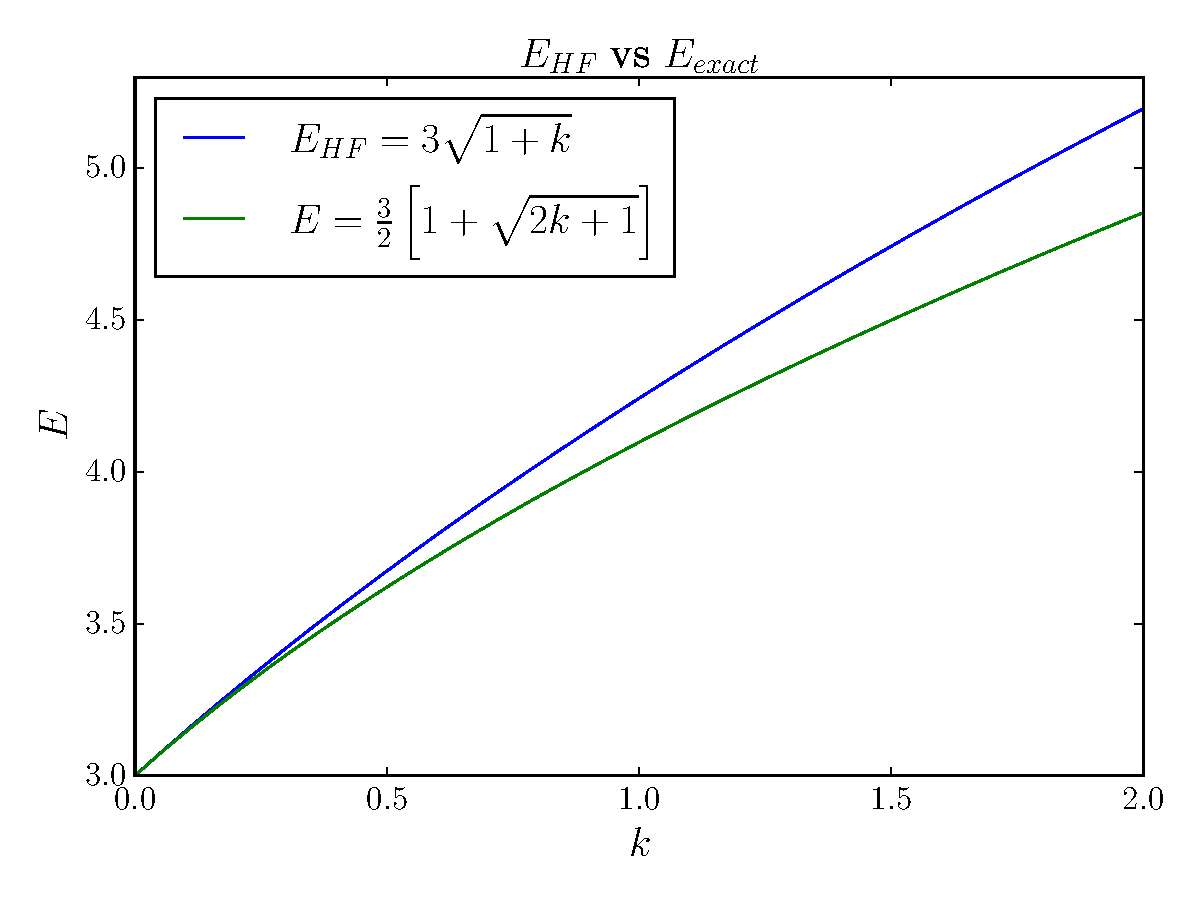
\includegraphics[width=0.45\textwidth]{3/img/HF_vs_excat}
    \caption{Graphical comparison between the energy computed by HF and the analytic solution
    for the same system \cite{Moshinsky}.}
\label{HF_vs_excat}
\end{wrapfigure}

\noindent with the wavefunctions, respectively:

\begin{align}
  \psi = \pi^{-3/2} (2\kappa +1)^{3/8} e^{-\frac12 R^2} e^{-\frac12(2\kappa+1)^{1/2}r^2} \\\nonumber
  \psi_{HF} = \pi^{-3/2}(\kappa +1)^{3/4} e^{-1/2(\kappa +1)^{1/2}(r^2+R^2)}
\end{align}

In Figure \ref{HF_vs_excat} it is possible to see how the analytic solution and
the Hartree Fock approach are close at small $\kappa$ values. For the energy it
is possible obtain 95 \% of the exact energy, but just the 65 \% for the
overlap. In Figure \ref{HF_vs_psi} it is possible to see how the HF
wavefunction moves away from the exact solution as $\kappa$ increases.

%\newpage

\begin{figure}
  \centering
  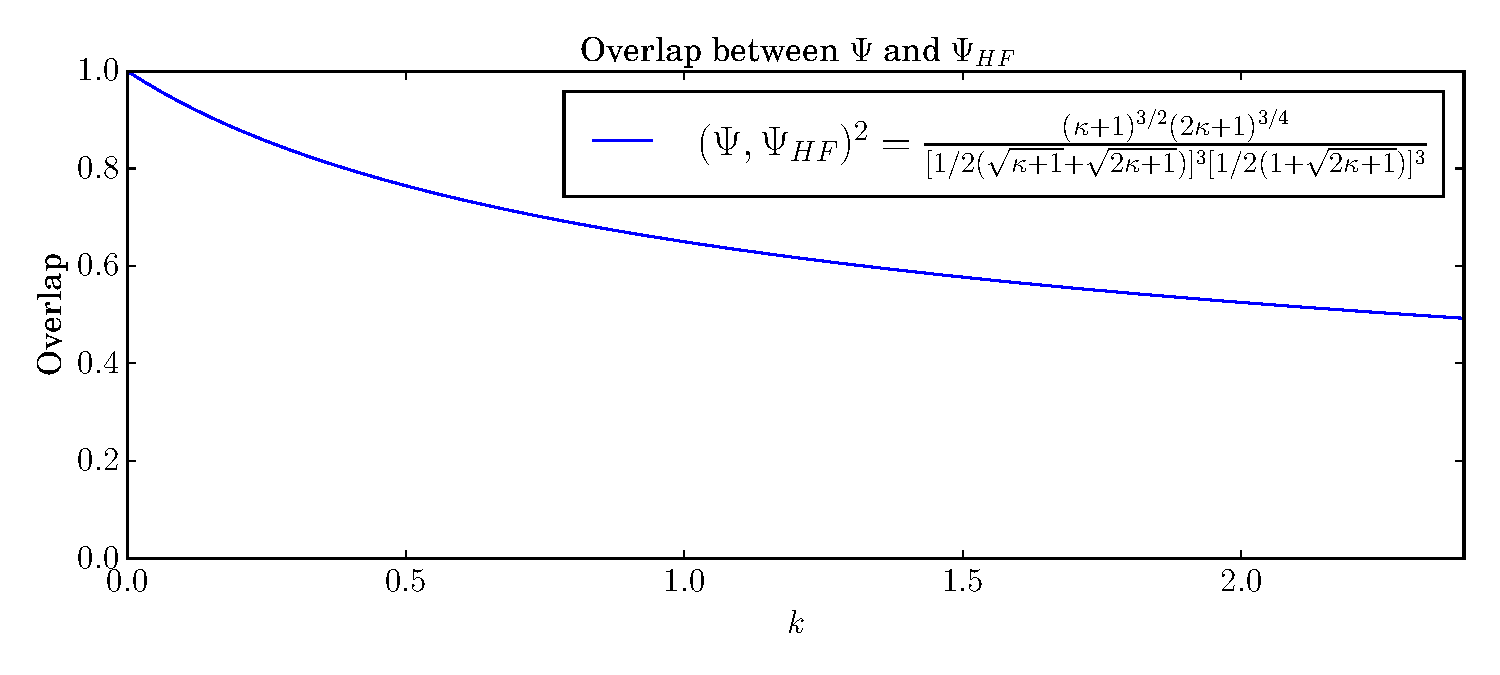
\includegraphics[width=1\textwidth]{3/img/HF_vs_psi.pdf}
  \caption{Overlap as a function of parameter $k$.}
\label{HF_vs_psi}
\end{figure}

Therefore, using HF for quantum chemistry can be a cheap and meaningful way in
computational terms, functional for small systems with low correlation, as it
is shown with small $\kappa$ values in the previous system, \textit{e.  g.} the
optimization of the equilibrium distance for H$_2$ or CH$_4$
\cite{defrees1982effect}.

\pagebreak

In contrast, HF fails for dissociation processes where the total spin value is
not conserved as the nuclear coordinates change~\cite{JimnezHoyos2012}.  Some
other problems that HF has are: $i$) it does not respect the Pauli's exclusion
postulate, $ii$) in Central Field Approximation (\gls{CFA}) the spherical
harmonics are not necessary eigenfunctions of the monoelectronic equation,
$iii$) there is not an obvious way to improve the orbital approach, and $iv$)
it does not consider correlation effects, which are not necessarily despicable
in all cases.

\section{Electronic Density}\label{densidades}

One of the most important terms to define in theoretical chemical physics is
the electronic density $\rho (\vec{r})$, which for a system of two electrons
with spin-spatial coordinates $\vec{x}_{1}$ and $\vec{x}_2$, is defined as:
$|\Psi (\vec{x}_1 ,  \vec{x}_2)|^2$~\cite{RobertG1994}.  To compute the
probability to find simultaneously the electron 1 in $d\vec{x}_1$ and 2 in
$d\vec{x}_2$, it is necessary to integrate the density function over $d\omega_1
d\vec{x}_2$, where: $d\vec{x}_n =  d\vec{r}_n d\omega_n$,

%
\begin{align}
  P(\vec{r}_1)=\int |\Psi (\vec{x}_1 ,  \vec{x}_2)|^2 d\omega_1 d\vec{x}_2 ,
\end{align}

\noindent and, since the electrons are indistinguishable, we obtain the following expression:
%
\begin{align}
  \rho(\vec{r})=2\int |\Psi (\vec{x}_1 ,  \vec{x}_2)|^2 d\omega_1 d\vec{x}_2 ,
\end{align}

\noindent Then, for a system with $N$ electrons, the electronic density can be
generalized as follows:
%
\begin{align}
  \rho(\vec{r})=N\int |\Psi (\vec{x}_1 ,  \vec{x}_2,  \ldots , \vec{x}_N)|^2
  d\omega_1 d\vec{x}_2 \ldots d\vec{x}_N ,
\label{definition}
\end{align}

\noindent such that:
%
\begin{align}
  \int\rho (\vec{r})d\vec{r} =N ,
\end{align}

\noindent In the case of a Slater Determinant (Hartree-Fock), it is possible to write
the electronic density for a closed shell with spacial orbitals ${\psi_a}$ as:
%
\begin{align}
  \rho (\vec{r}) = 2 \sum_{a=1}^{N/2} |\psi_a (\vec{r})|^2 
\end{align}

For a system with $N$ particles, it is possible to write an operator for the
density $\hat{\rho}$ and then, get the expected value for the system
wavefunction,
%
\begin{align}
  \hat{\rho} = \sum_i ^N \delta (\hat{r}_i - \vec{r}_0),
\end{align}

\noindent then $\rho (\vec{r})$ is a expected value of a quantum mechanics
operator, which can be written as:
%
\begin{align}
  \rho (\vec{r})= \int\Psi^{\star} (\vec{x}_1, \ldots , \vec{x}_N)
  \sum_i ^N \delta (\hat{r}_i - \vec{r}_0) \Psi (\vec{x}_1, \ldots , \vec{x}_N)
  d\vec{x}_1 \ldots d\vec{x}_N 
\end{align}

The value of the electronic density is very important, since it is a value that
can be obtained from experimental data. The experiments from which we can
obtain $\rho (\vec{r})$ information are the X-Ray diffraction or neutron
diffraction~\cite{Kasai2018, Coppens1971}.  Thus, we can compare the
theoretical values with experimental data, and have an idea of how good are the
theoretical considerations for the computation.

However, it is also possible to establish a density function for an electron
couple, also called pair density, such that:
%
\begin{align}
  \rho_2(\vec{r_1},\vec{r_2})=N(N-1)\int |\Psi (\vec{x}_1 ,  \vec{x}_2,  \ldots , \vec{x}_N)|^2
  d\omega_1 d\omega_2  d\vec{x}_3 \ldots d\vec{x}_N ,
\label{d_pares}
\end{align}

\noindent where $\rho_2(\vec{r}_1,\vec{r}_2)N^{-1}(N-1)^{-1}$ determines the
probability of simultaneously finding two electrons per volume centered at
positions $\vec{r_1}$ and $\vec{r_2}$, commonly expressed by a sum which
involves independent pairs terms and correlations, $\rho_2(\vec{r}_1,
\vec{r}_2) = \rho(\vec{r}_1)\rho(\vec{r}_2) + \rho_2^{xc}(\vec{r}_2,
\vec{r}_1)$.

The relevance of the electron and the pair densities (Equations
\ref{definition} and \ref{d_pares}, respectively) comes from the fact that the
energy of the system within the Born-Oppenheimer approximation and in the
absence of external fields can be expressed in terms of these two densities:
%
\begin{align}
  E=&-\frac{1}{2}\int\nabla^{2}\rho_{1}(\vec{r}_1,
    \vec{r}^{\,\prime}_1) \biggr |_{\vec{r}^{\,\prime}_1 \rightarrow \vec{r}_1}
    d\vec{r}_1 -\sum_{A}\int\frac{Z_A \rho_1 (\vec{r}_1)}{r_{1A}}d\vec{r}_1
    +\sum_{A\neq B}\frac{Z_A Z_{B}}{r_{AB}} \nonumber \\
  \phantom{=}&+\frac{1}{2}\int\int\frac{\rho (\vec{r}_1) \rho
    (\vec{r}_2)}{r_{12}} d\vec{r}_1 d\vec{r}_2
    -\frac{1}{2}\int\int\frac{\rho_2^{xc}(\vec{r}_1, \vec{r}_2)}{r_{12}} d\vec{r}_1
    d\vec{r}_2 \nonumber \\
  =&\ T + V_{ne} + V_{nn} + V_{ee} + V_{xc}
\label{E_b-o}
\end{align}

\noindent where the first term is the kinetic energy, the second and the third
terms are the nucleus-electron and nucleus-nucleus energy from Born-Oppenheimer
approximation. Then the electron-electron repulsion is computed by the product
of densities. Finally, the last term, the pair density, it is used to compute
the exchange-correlation phenomenon.  Subtracting the product between
$\rho(\vec{r_1})$ and $\rho(\vec{r_2})$ from the pair density we have the
information of the exchange-correlation phenomenon, since this term contains
all the information about the indistinguishability of electrons and how one of
the electrons is conditioned by the other one.

In practice, Equation \ref{E_b-o} for a electronic structure method requires to
express the density distribution as a function of the molecular orbital basis,
$\phi_i$,
%
\begin{align}
  \rho_1 (\vec{r}) = \sum_{ij} D_{ij}\phi_{i}(\vec{r})\phi_{j}(\vec{r}),
\end{align}
\begin{align}
  \rho_2 (\vec{r}_1, \vec{r}_2) = \sum_{ijkl}d_{ijkl}\phi_{i}(\vec{r}_1) \phi_{j}(\vec{r}_1)
  \phi_{k}(\vec{r}_2)\phi_{l}(\vec{r}_2),
\end{align}

\noindent where $D_{ij}$ and $d_{ijkl}$ are the matrix elements of the first
and second order density matrix.

\subsection{Density matrix}

We know that the expected value for any operator can be obtained as:
%
\begin{align}
	\begin{split}
    \langle \widehat{Q} \rangle & = \int\Psi^{\star}(x_{1},x_{2},\ldots,x_{n}) \widehat{Q}
    \Psi(x_{1},x_{2},\ldots,x_{n}) dx_{1}\ldots dx_{n} \\ 
	  & = \int\widehat{Q}\Psi(x_{1},x_{2},\ldots,x_{n}) \Psi^{\star}(x^{\prime}_{1},x^{\prime}_{2},\ldots,x^{\prime}_{n})
	  dx_{1}\ldots dx_{n} ,
	\end{split}
\end{align}

\noindent with emphasis on the fact that the operator does not act for the
primed variables.

If we have an operator that involves $m$ variables, with $m\le n$, we can
write:
%
\small
\begin{align}
	\begin{split}
\langle \widehat{Q} \rangle & = \int\widehat{Q}\Psi(x_{1},\ldots , x_{m}, x_{m+1}, \ldots , x_{n})
\Psi^{\star}(x_{1},\ldots , x_{m}, x_{m+1}, \ldots , x_{n}) dx_{1}\ldots dx_{n} \\
	& =\int dx_{1}\ldots dx_{m} \widehat{Q}\int\Psi(x_{1},\ldots , x_{m}, x_{m+1}, \ldots , x_{n})
	\Psi^{\star}(x_{1},\ldots , x_{m}, x_{m+1}, \ldots , x_{n}) dx_{m+1}\ldots dx_{n}\\
	& =\int dx_{1}\ldots dx_{m} \widehat{Q} (x_{1}, \ldots , x_{m}) F_{m}
	(x_{1}, \ldots , x_{m}; x^{\prime}_{1}, \ldots , x^{\prime}_{m}),
	\end{split}
\end{align}
\normalsize

\noindent with:
%
\footnotesize
\begin{align}
  F_{m}(x_{1}, \ldots , x_{m}; x^{\prime}_{1}, \ldots , x^{\prime}_{m}) =
  \int dx_{m+1}\ldots dx_{n} \Psi(x_{1},\ldots , x_{m}, x_{m+1}, \ldots , x_{n})
  \Psi^{\star}(x^{\prime}_{1},\ldots , x^{\prime}_{m}, x^{\prime}_{m+1}, \ldots , x^{\prime}_{n})
\end{align}
\normalsize

The $F$ function can be related to the density matrix
$\Gamma$ at order $m$ defined by:
%
\footnotesize
\begin{align}
  \Gamma_{m}(x_{1}, \ldots , x_{m}; x^{\prime}_{1}, \ldots , x^{\prime}_{m}) = {n \choose m}\int dx_{m+1}
  dx_{n} \Psi^{\star}(x^{\prime}_{1},\ldots , x^{\prime}_{m}, x^{\prime}_{m+1}, \ldots , x^{\prime}_{n}) \Psi(x_{1},\ldots ,x_{n}),
\end{align}
\normalsize

\noindent where ${n \choose m}$ are the combinations of $n$ elements taken in
$m$
 
%
\small
\begin{align}
  {n \choose m} = \frac{n!}{m! (n-m)!}\, 
\end{align}
\normalsize

There is a hierarchy between the density matrix 
according to their order,
\small
\begin{align}
  \begin{split}
  \Gamma_{m}(x_{1}, \ldots , x_{m}; x^{\prime}_{1}, \ldots , x^{\prime}_{m}) & = \frac{{n \choose m}}{{n \choose {m+1}}}
  \int dx_{m+1}\Gamma_{m+1}(1, \ldots , m, m+1;1^{\prime}, \ldots , m^{\prime}, (m+1)^{\prime}) \\
	  & = \frac{m+1}{n-m} \int dx_{m+1}\Gamma_{m+1}(1, \ldots , m, m+1;1^{\prime}, \ldots , m^{\prime}, (m+1)^{\prime})
  \end{split}
\end{align}
\normalsize

Since in quantum chemistry the operators are mono- or bi-electronic, the
density matrices with useful information are the first and second order density
matrices. There are two normalization criteria, $\frac{n(n-1)}{2}$ or $n(n-1)$,
exposed by L\"owdin and McWeeny  respectively~\cite{Lwdin1955,mcweeny},
%
\begin{align}
  \Gamma_{1} (x_1;x_1^{\prime}) = n\int\Psi^{\star}(1^{\prime}, 2^{\prime}, \ldots ,n^{\prime})\Psi(1, 2, \ldots , n) dx_{2} \ldots dx_{n}
\label{m_primer_orden}
\end{align}
\begin{align}
  \Gamma_{2} (x_{1}, x_{2};x^{\prime}_{1},x^{\prime}_{2}) = \frac{n(n-1)}{2} \int\Psi^{\star}(1^{\prime}, 2^{\prime}, \ldots ,n^{\prime})
  \Psi(1, 2, \ldots , n) dx_{3} \ldots dx_{n}
\end{align}

For many applications it is convenient to work with the first order density
matrix, also called Fock-Dirac (Equation \ref{m_primer_orden}), and when it is
integrated with respect to the spin coordinate it gives the first order reduced
matrix,

%
\begin{align}
  \rho_{1}(r_{1},r^{\prime}_{1}) = \int\Gamma_{1} (x_{1};x_{1}^{\prime})
\label{m_r_1}
\end{align}

\noindent Unlike the density functions, the matrix elements have no physical
meaning, except for the diagonal ones, which in the case of the first order
reduced matrix coincides with the electronic density.

It is important to highlight that the sum of the elements of the first order
density matrix, which is an integral because of the continuous nature of the
matrix indices, is equal to the total number of the electrons of the system.

Hence, many properties of the polyelectronic systems, and particularly the
energy, can be expressed as a function of the first order density matrix and
bi-electronic density.

\section{Density Functional Theory}

Before starting with the Density Functional Theory, it would be helpful to know
about functionals, a term that has many definitions. For theoretical physics
and chemistry the functionals are really useful, the main idea is that the
functional does not depend on a scalar, vector, matrix or tensor at any order,
but on a function; and it renders a number.

This idea is very useful to explore concepts such as the functional derivative,
useful in Lagrange mechanics, or the functional integrals which are the central
idea behind the path integrals exposed by Richard Feynman.

The three most common definitions used to describe a functional are~\cite{1990}:

\begin{itemize}
\item In linear algebra, it makes reference to a linear mapping from a vector
space $V$ into its field of scalars, that is, an element of the dual space
$V^{*}$.
\item In functional analysis and related fields, it refers more generally to a
mapping from a space $X$ into the real or complex numbers. In functional
analysis, the term linear functional is a synonym of linear form; that is, it
is a scalar-valued linear map. Depending on the author, such mappings may or
may not be assumed to be linear, or to be defined on the whole space.
\item In computer science, it is synonymous of higher-order functions, that is,
functions that take functions as arguments or return them.
\end{itemize}

Clarified the functional term, we can start with a brief summary of Density
Functional Theory, which is one of the most important theories used in
theoretical physical chemistry. Where the \citet*{Hohenberg1964} and
\citet*{Kohn1965} papers are among the most cited papers until now, which will
be covered in Sections \ref{HKteoremitas} and \ref{KSapprox}.

It is worth noting that it is a variational method where the functional of the
electronic energy is minimized with respect of the electronic density. This is
a really important step, because we are not using anymore the wavefunction
\textit{per se}, which leads to some computational benefits to solve big
systems.

\pagebreak

The electronic density is a scalar magnitude easier to compute because it
depends just on three spacial variables, unlike the wavefunction which depends
on 3$N$ variables. However, except for the easiest cases, DFT has the
inconvenience that although although there exists an exact functional that
provides the exact energy of the system, its form is unknown.

This way of understanding the Quantum Mechanics is a clear exhibition of the
Copenhagen interpretation.  One of the principal drawbacks of DFT is that even
being a exact theory, it can be only applied approximately, because of this
there is not a systematic way of knowing how close the result is to the exact
value. 

Additionally, the exchange interaction is not correctly treated, thus the
exchange-correlation energy can be very different depending of how the
calculation is approached.

Due to the above and some other perspectives, there is a scientific community
division, between defenders and detractors. On the one hand, defenders claim
that the results are really good for the computational cost and it is a good
way to approach big systems; on the other hand, the detractors argue that the
results are not as reliable as a classical \textit{ab initio} treatment.

Historically, the first approaches to obtain information of a system using the
electronic density started in 1927 with Llewellyn Hilleth Thomas and Enrico
Fermi works~\cite{Thomas1927,fermi1927statistical}. The main idea is to take
the kinetic energy in terms of the nucleus-electron and electron-electron
contributions, purely treated as classical interactions, in a uniform
electronic gas. Let a fictitious system be with a constant electronic density:

\begin{align}
  {T}_{\mathrm{TF}}[\rho(\vec{r})]=\displaystyle\frac{3}{10}(3\pi^2)^{(2/3)}\int
  \rho^{(5/3)}(\vec{r})d\vec{r}
\end{align}

Combining $T_{HF}$ with the above mentioned contributions, we obtain an
expression for the Thomas-Fermi atomic energy. This approximation, shown in
Equation \ref{E_TF}, works quite well for alkaline metals and moderately well
for alkaline-earth metals:
%
\begin{align}
  {E}_{\mathrm{TF}}[\rho(\vec{r})]=\displaystyle\frac{3}{10}(3\pi^2)^{(2/3)}\int
  \rho^{(5/3)}(\vec{r})d\vec{r}-Z\int\displaystyle\frac{\rho(\vec{r})}{r}d\vec{r}
  +
  \displaystyle\frac{1}{2}\int\int\displaystyle\frac{\rho(\vec{r_1})\rho(\vec{r_2})}{r_{12}}
  d\vec{r_1}d\vec{r_2}
\label{E_TF}
\end{align}

This way of approaching quantum mechanical problems became significantly
important in 1964 when Hohenberg and Kohn published their
theorems~\cite{Hohenberg1964}. More specifically $i$) the energy is a
functional of the density and $ii$) the density of a system minimizes the
functional.

Another big step in DFT was published by Kohn and Sham one year
after~\cite{Kohn1965}, and it says that it is possible to write an equation for
orbitals of a particle, from which the density can be obtained.

Nowadays, this method is widely used; however, in the early days it was used
more in solid physics, since it was not considered a method accurate enough to
be applied to chemistry.  Although if originally DFT did not contemplate
temporal dependency, it was introduced using relativistic quantum mechanics,
being denoted as \gls{TDDFT} (Time-dependent Density Functional Theory).

In 1984, a generalization of the Hohenberg-Kohn theorems was published, carried
out by Runge and Gross for the case of the time dependency. It states that
there is a one-to-one relationship between the time dependent density $\rho
(\vec{r}, t)$ and the external potential of a body $v_{ext} (\vec{r}, t)$ to an
initial state~\cite{Runge1984}. Unlike DFT, there is not a general minimization
principle in time dependent quantum mechanics, therefore its proof is more
complicated.

%\newpage

\subsection{Hohenberg-Kohn Theorems}\label{HKteoremitas}
\subsubsection{Theorem 1~\cite{Hohenberg1964}}

The energy, and therefore, the rest of the system properties, are unequivocally
determined by the electronic density. If two systems with $N$ particles are in
external fields $v_{1} (\vec{r})$ and $v_{2} (\vec{r})$, with the same
electronic density at the ground state $\rho(\vec{r})$, the difference between
$v_{1} (\vec{r})$ and $v_{2} (\vec{r})$ is necessarily a constant. Therefore,
there cannot be two potentials to describe the same ground state.

Corollary: the potential and all system properties are uniquely determined
through the density of the fundamental state, including the many-body
wavefunction of the state. Particularly, the \gls{HK} functional is defined as
$F[\rho]=T[\rho]+U[\rho]$ (universal density functional), which does not
strictly depend on an external potential.

\pagebreak

The value of the ground state of any observable is a unique function of the
exact electronic density of the ground state given by:
\begin{align}
  \langle \psi |\widehat{A}|\psi \rangle = A[\rho_0 (r)]
\end{align}

\subsubsection{Theorem 2}

The functional that gives the ground state energy gives the lowest energy, if
and only if, the density that gives the functional is the true density of the
ground state. \textit{i. e.,} the energy obtained from the Hamiltonian is the
absolute minimum when the electron density of the ground state is used.

For any potential $v_{ext}(\vec{r})$ and natural $N$, the density function
$F[\rho]$ exists as:
%
\begin{align}
  E_{v, N} [\rho] = F[\rho] + \int v_{ext}(\vec{r})\rho(\vec{r}) d^{3}r ,
\end{align}

\noindent and the minimum value is obtained in the ground state density for $N$
electrons with the potential $v_{ext}(\vec{r})$. The minimum value of $E_{v, N}
[\rho]$ is then the energy of the ground state of the system.

The second theorem establishes that the exact value of the energy is a minimum
value of the functional, \textit{i. e.}, we have an inferior limit for the
calculation.  Thus, there is a variational principle for the energy,
%
\begin{align}
  E_{0}\leq E[\rho]=T[\rho] + V_{Ne}[\rho]+V_{ee}[\rho]
\end{align}

\subsection{Kohn-Sham Approximation}\label{KSapprox}

Kohn and Sham proposed a new approximation to solve the problem of many
electrons based on the HK theorems. The total energy of the external potential
functional $v_{ext}(\vec{r})$ can be described by:
\begin{align}
  E[\rho(\vec{r})] = T[\rho(\vec{r})] + \int v_{ext}(\vec{r})\rho(\vec{r})d^{3}r +
  V_{ee}[\rho(\vec{r})] 
  \label{KS1}
\end{align}
\noindent with:
\begin{align}
  V_{ee}[\rho(\vec{r})] = \frac12 \int\int \frac{\rho(\vec{r})\rho(\acute{r})}{|\vec{r}-\acute{r}|}d^{3}r
  d^{3}\acute{r} + {E}_{xc}[\rho(\vec{r})] 
\end{align}

The first term of Equation \ref{KS1} is the kinetic energy $T[\rho(\vec{r})]$,
the second one is the external potential given by the nuclei arrangement, and
the last one is the classic and non-classical contributions (exchange
correlation behind of the mean field theory of electron-electron interaction).
To solve the Kohn-Sham equations it is necessary to assume a reference system
with non-interacting particles with the same density as the ground state
interacting system. Thus, we can write the next equation for the system:

\begin{align}
  \left [-\sum_{i}\frac12\nabla^{2}_{i} + v_{eff}[\rho(\vec{r})]\right ]|
%E_{eff}|\psi_{i}\rangle = \left [-\sum_{i}\frac12\nabla^{2}_{i} + v_{eff}[\rho(\vec{r})]\right ]|
  \psi_{i} \rangle =
  \epsilon_{i}|\psi_{i}\rangle ,
\end{align}

\noindent where the subscript $eff$ means effective, hence $v_{eff}$ means
effective potential in the non-interacting system.  We thus have an expression
for the kinetic energy of the non-interacting system:
\begin{align}
  T_{eff}[\rho(\vec{r})] = \sum_{i}\epsilon_{i} - V_{eff}[\rho(\vec{r})]
%T_{eff}[\rho(\vec{r})] = \sum_{i}n_{i}\epsilon_{i} - V_{eff}[\rho(\vec{r})].
\end{align}

The new pseudo-kinetic-energy is used to compute the exchange-correlation functional of the energy
$E_{xc}[\rho(\vec{r})]$ which is expressed as:
\begin{align}
E_{xc}[\rho(\vec{r})] = T[\rho(\vec{r})] - T_{eff}[\rho(\vec{r})] +
V_{ee}[\rho(\vec{r})] - J[\rho(\vec{r})] 
\end{align}

Using $i$) the new exchange-correlation functional of the total energy of the system,
$ii$) differentiating the new total non-interactive energy and the effective
potential with respect to the electronic density $\rho(\vec{r})$, and $iii$)
the Schrödinger Equation for an electron moving in a
potential $v_{eff}$:

\begin{align}
  \left[-\frac12\nabla^2 + v_{eff}[\rho(\vec{r})]\right]\psi_{i}(\vec{r})=\epsilon_{i}\psi_{i}(\vec{r})
\end{align}

\vspace{5mm}
We have the energy of the interacting system:
\begin{align}
  E[\rho] = \sum_i\epsilon_i -\frac12\int\int\frac{\rho(\vec{r})\rho(\acute{r})}
  {|\vec{r}-\acute{r}|}d^3r d^3\acute{r}+ E_{xc}[\rho(\vec{r})] -
  \int\frac{\delta E_{xc}[\rho(\vec{r})]}{\delta\rho(\vec{r})}\rho(\vec{r})d^3r 
%E_{0}=\sum_{i}n_{i}\epsilon_{i} -\int\int\frac{\rho(r)\rho(\acute{r})}
%{|r-\acute{r}|}d^3r d^3\acute{r}+
%E_{xc}[\rho(\vec{r})] .
%V_{eff} = V_{Ne}(\vec{r}) + \int\frac{\rho(\vec{r})}{|\vec{r}-\acute{r}|}d^3 r
%+ V_{xc}(\vec{r}) .
\end{align}

\subsection{Exchange-Correlation Functionals}

There are many types of functionals for exchange-correlation inside DFT and it
is possible to classify them by the approximations that are used in their
construction:
%
\begin{itemize}
\item \textbf{Local Density Approximation (LDA)}. In LDA the density is shaped
as a local homogeneous electronic gas, with electronic density $\rho$. In this
system, the electrons move in a distribution of positive charges, additionally,
the gas is electrically neutral and with an infinite volume which contains an
infinite number of non-interacting electrons~\cite{Koch2001}.

$E_{xc}^{LDA} [\rho] = \int \rho (r) \varepsilon_{xc}(\rho (r)) dr$

Taking the functional derivative of $E_{xc}^{LDA}$ we obtain:

$v_{xc}^{LDA} = \frac{\delta E_{xc}^{LDA}}{\delta\rho} = \varepsilon_{xc}(\rho (r))
+ \rho \frac{\partial \varepsilon_{xc}(\rho (r))}{\partial\rho}$

where $\varepsilon_{xc}$ can be decomposed in the contributions of exchange and
correlation, with the expression for $\varepsilon_{x}$ as:

$\varepsilon_{x} = -\frac34 \left( \frac{3}{\pi} \right)^{\sfrac13}\rho^{\sfrac13}$ 

Functionals developed in LDA approach have different ways to improve the
results. The X$_{\alpha}$ method~\cite{Slater74} has an empiric value $\alpha$,
The Local Spin Density Approximation (LSDA)~\cite{Slater74} is used to spin
polarized system through the employment two spin-densities ($\rho_\alpha$,
$\rho_\beta$).

Unfortunately, there is no known analytical expression for the correlation
energy ($\varepsilon_{cor}$). Nevertheless, some studies was developed with
Quantum Monte-Carlo by Vosko, Wilk and Nussar, as published in the functional
VWN~\cite{Vosko1980}. Another way to approach the correlation problem was done
by Perdew and Zunger, they used the values from Ceperley and
Alder~\cite{Ceperley1980} to adjust an expression that fulfill the conditions
at low and high densities in their functional PL~\cite{Perdew1981}.


\item \textbf{Generalized-Gradient Approximation (GGA)}.  In \gls{GGA}
approximation is aim to correct the density constant introducing the density
gradient.

$E_{xc}^{GGA} [\rho] = \int \rho (r) v_{xc}(\rho (r), \nabla\rho (r)) dr$

As in LDA case, the energy $E_{xc}^{GGA}$ can be decomposed in the exchange
and correlation contributions.

There are many ideas to insert the gradient, one of those was proposed by
Becke, incorporating the concept of correlation hole for its formulation, Becke
published sundry functionals, but one of the most famous is
B88~\cite{Becke1988}. While other GGA functionals were developed as an
improvement of an previous GGA functional, as the mPW
functional~\cite{Adamo1998}, where is improved the long-range behavior.

The functional B88 is frequently accompanied by the correlation functional
LYP~\cite{Lee1988}, which is a correlation functional that considers the term
of Weizsacker kinetic energy~\cite{weizsacker1935theorie} to transform the
Colle and Salvetti functional~\cite{Colle1975} (correlation for closed shells).

Another popular functional in GGA approach is P86 developed with the idea of
the natural separation between exchange and correlation, thus the
density-gradient expansion of each is recovered in the slowly varying limit.
Also the uniform-gas and inhomogeneity effects beyond the random phase
approximation are built in~\cite{Perdew1986}. The gradient dependent term is
neglected for uniform densities, therefore, the functional recover the local
form for uniform electron gases.


\item \textbf{Meta-Generalized Gradient Approximation (meta-GGA)}.  In meta-GGA
the Laplacian of the density is also included, $\nabla^{2}\rho (r)$. This
allows to obtain a better description of the system.  In practice the kinetic
energy density is used, where the sum is over the \gls{KS} occupied orbitals.

$\tau (r) = \displaystyle\sum_{i}^{N} \displaystyle\frac12 |\nabla\psi_i (r)|^{2}$

$E_{xc}^{MGGA} [\rho] =\int\rho (r) v_{xc}(\rho (r), \nabla\rho (r), \tau (r)) dr$

The kinetic energy density and the Laplacian are related by the external potential:

$\tau (r) = \displaystyle\sum_{i}^{N} \displaystyle\frac12 \varepsilon_i |\psi_i (r)|^{2}
- v(r)\rho(r) + \displaystyle\frac12 \nabla^2\rho(r)$

The use of the Laplacian is computationally expensive, and for a long time
the performance was not much improved. Some new functionals (\textit{e. g.}
SCAN~\cite{scan}) have shown nevertheless an important improve over GGAs.

Two popular meta-GGA functionals are: $i$) the VSXC
functional~\cite{VanVoorhis1998} which approach the meta-GGA through the
density matrix expansion, and $ii$) the KCIS functional~\cite{1999} which
propose an accurate self-interaction-corrected correlation with a gap on the
electron gas.


\item \textbf{Hybrid Functionals}.  These functionals include one part of the
exact exchange energy at Hartree-Fock level, which is computed with the
Kohn-Sham orbitals.

$E_{x}^{HF} [\theta_{i}] = -\displaystyle\sum_{i=1}^{N/2}\displaystyle\sum_{j=1}^{N/2}
\displaystyle\frac{\theta_{i}^{\star}(r_{1}) \theta_{j}^{\star}(r_{1}) \theta_{i}(r_{2}) \theta_{j}(r_{2})}
{r_{12}} dr_{1}dr_{2}$

The most popular hybrid functional is B3LYP, it was built for the first time in
1994, combining Becke's three-parameter hybrid functional~\cite{Becke1993} with
correlation functional LYP~\cite{Lee1988}. Following the next equation:

$E_{xc}^{B3LYP} = aE_{x}^{Slater} + (1-a)E_{x}^{HF} +bE_{x}^{Becke88}
+cE_{c}^{LYP} +(1-c)E_{c}^{VWN}$,\\

where $a$=0.80, $b$=0.72 and $c$=0.81 are empirical parameters adjusted to the
ionization, enthalpy of atomization, proton affinity and atomic energies.

Other examples of hybrid functionals are PBEh1PBE~\cite{Ernzerhof1998} and
M06-2X~\cite{Zhao2007}. 

\end{itemize}

In this work the M06-2X functional is used in the majority of calculations,
which is a Hybrid Functional belonging to the functional series developed by
Zhao and Truhlar at the University of Minnesota~\cite{Zhao2007}. These
functionals were developed taking empirical parameters, but still thinking in
the free electron gas model.

The functional is a hybrid meta-GGA with high delocalization, containing 54 \%
of Hartree Fock exchange. Also it depends on three variables which are $i$) the
spin density, $ii$) the reduced gradient of the density,
\begin{align}
  x_{\sigma} = \frac{|\nabla \rho_\sigma|}{\rho^{\sfrac43}_{\sigma}}, \, \sigma=\alpha,\beta,
\end{align}
and $iii$) the spin kinetic energy $\tau_\sigma$.

The functional M062X includes terms based on the functional
VSXC~\cite{VanVoorhis1998}, which contains the variable  $z_\sigma$ and the
functions $\gamma$ and $h$, as well as an empiric constant $C_F$, defined as:

\begin{align}
  \begin{split}
    z_\sigma &= \frac{2\tau_\sigma}{\rho_\sigma^{\sfrac53}} - C_F\\
    C_F &= \frac35 \left( 6\pi^2 \right)^{\sfrac23}\\
    \gamma(x_\sigma, z_\sigma ) &= 1 +\alpha (x_\sigma^2 +z_\sigma)\\
    h(x_\sigma, z_\sigma ) &=
    \left( \frac{d_0}{\gamma(x_\sigma, z_\sigma )} + \frac{d_1x\sigma^2 + d_2z_\sigma}{\gamma^2(x_\sigma, z_\sigma )} + \frac{d_3x_\sigma^4 + d_4x_\sigma^2z_\sigma + d_5z_\sigma^2}{\gamma^3(x_\sigma, z_\sigma )} \right) 
  \end{split}
\label{h_de_M062X}
\end{align}

\noindent where $\alpha$, $d_i (i=0,...,5)$ are parameters adjusted to
experimental data.

The exchange part of M062X came from a linear combination between M05 and
VSXC~\cite{Zhao2007}.

\begin{align}
  E_X^{DFT} = \sum_\sigma \int
  \left( F_{X_\sigma}^{PBE}(\rho_\sigma,\nabla\rho_\sigma) f(w_\sigma) + \varepsilon_{X_\sigma}^{LSDA}h_X (x_\sigma, z_\sigma) \right) d\mathbf{r},
\end{align}

\noindent where $F_{X_\sigma}^{PBE}(\rho_\sigma,\nabla\rho_\sigma)$ is the
exchange energy density from PBE~\cite{Zhao2007},
$\varepsilon_{X_\sigma}^{LSDA}$ is the exchange energy per particle in the
\gls{LSDA} approximation, $f(w_\sigma)$ is a correction factor of the density
of spin kinetic energy, and $h (x_\sigma, z_\sigma)$ was already defined in
Equation \ref{h_de_M062X}.  That last term is peculiar in M062X, since M062X
takes the exchange part from M05, $h_X (x_\sigma, z_\sigma) = 0$
\cite{Zhao2007,Zhao2005}.

The correlation part is composed of two terms, one with opposite spins
$E_C^{\alpha\beta}$ and another one with parallel spins ($E_C^{\sigma\sigma}$),
in where $h (x_\sigma, z_\sigma)$ is not zero as in the exchange part:

\begin{align}
  E_C^{\alpha\beta} &= \int\varepsilon^{\mathrm{GEH}}_{\alpha\beta}
  \left[ g_{\alpha\beta} (x_\alpha, x_\beta) + h(x_{\alpha\beta},z_{\alpha\beta})\right]
  d\mathbf{r}\\
  E_C^{\sigma\sigma} &= \int\varepsilon^{\mathrm{GEH}}_{\sigma\sigma}
  \left[ g_{\sigma\sigma} (x_\sigma) + h(x_{\sigma},z_{\sigma})\right]
  d\mathbf{r}
\label{Ecalpha}
\end{align}

\pagebreak

The functions $g_{\alpha\beta}$ and $g_{\sigma\sigma}$ in Equation
\ref{Ecalpha} include empirical parameters,
$h(x_{\alpha\beta},z_{\alpha\beta})$ and $h(x_{\sigma},z_{\sigma})$ are defined
in Equation \ref{h_de_M062X}, $D_\sigma$ is a auto-interaction correction
factor, and $\varepsilon^{\mathrm{GEH}}_{\alpha\beta}$ and
$\varepsilon^{\mathrm{GEH}}_{\sigma\sigma}$ are the correlation energies that
depend on spin.

The total correlation energy in M062X is given by:

\begin{align}
E^{DFT}_C = E^{\alpha\beta}_C + E_C^{\alpha\alpha} + E_C^{\beta\beta}
\end{align}

As mentioned before, M062X incorporates 54 \% of Hartree-Fock exchange,
therefore, the final expression for exchange-correlation energy at M062X is:

\begin{align}
E_C^{\mathrm{M062X}} = \frac{54}{100}E_X^{\mathrm{HF}} +
\left( 1- \frac{54}{100} \right)E_X^{DFT} + E_C^{DFT}
\end{align}

\section{Topology}

Before continuing with the theoretical background of this thesis, it is
necessary to take a short mathematical parentheses on topology, since following
topics are based on topology.

One of the awesome steps that the mathematicians made in the XIX century was
the division of ``\textit{geometriam situs}'' from geometry, giving rise to
topology as a new branch of math.

Euler was the first to approach a geometry problem in which structural
properties and not metrics were the key to find the solution~\cite{euler1736}.
Euler called that new branch as $geometriam$ $situs$, nowadays called topology,
name given by Johann Benedict Listing (Gauss's student) to mark the autonomy of
topology from geometry~\cite{listing}.

Many applications of topology were developed with time. Graph theory can give
optimized trajectories for flights, and is used in the version-control system
git developed by Linus Torvalds. Knot theory provides a way to relate the knots
at DNA and the knots in a rope. Hairy ball theorem in algebraic topology gives
as a corollary that there will always be a windless place in any planet.

\pagebreak

Currently, topology has a variety of results. One of them is the four colour
theorem, which is a good story because it was one of the first times that the
use of computers went beyond doing jobs like a huge calculator. The theorem
says that any map with continuous regions can be coloured with the maximum of
four colours avoiding any adjacent regions with the same
colour~\cite{4colores}.  We illustrate an example in Figure \ref{australia}.

\begin{figure}[h]
  \centering
  \begin{subfigure}[b]{0.28\linewidth}
    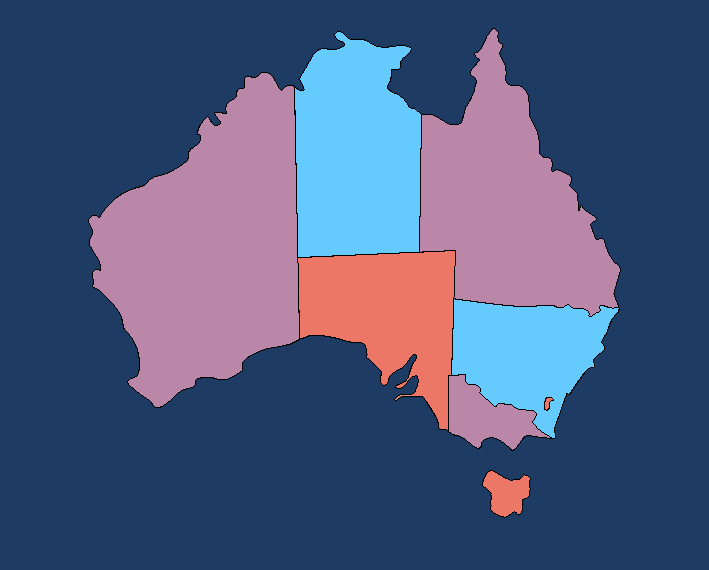
\includegraphics[width=\linewidth]{3/img/4_colors_australia_mapa}
    \caption{Australia map coloured with four colours.}
  \end{subfigure}
    \begin{subfigure}[b]{0.28\linewidth}
    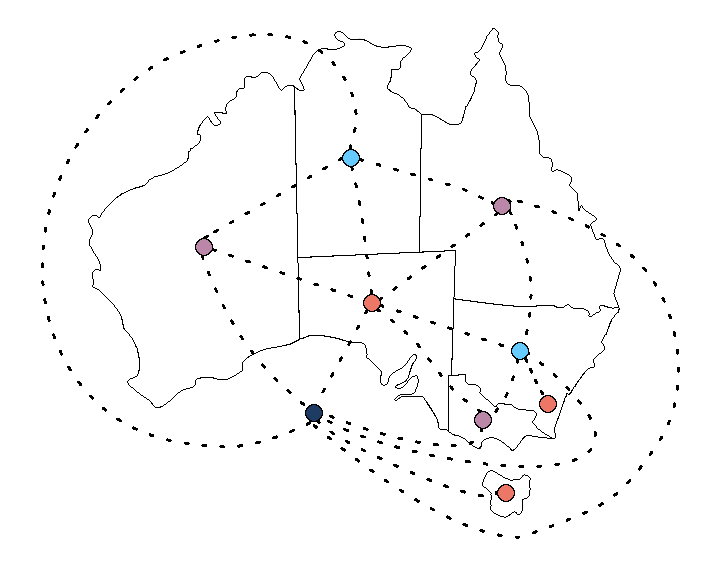
\includegraphics[width=\linewidth]{3/img/4_colors_australia_mapa_y_grafo}
    \caption{Australia map with its corresponding graph.}
  \end{subfigure}
    \begin{subfigure}[b]{0.28\linewidth}
    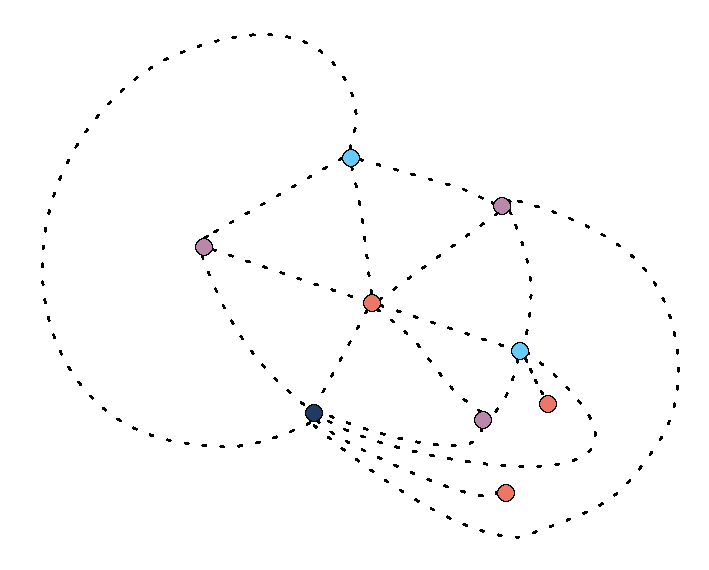
\includegraphics[width=\linewidth]{3/img/4_colors_australia_grafo}
    \caption{Graphic corresponding of the Australia map.}
  \end{subfigure}
  \caption{Example of the four colours theorem.}
  \label{australia}
\end{figure}

In 1976 Kenneth Appel and Wolfgang Haken proved the theorem by making 1936 maps
that are part of any counterexample to the theorem, the work to obtain the 1936
maps was hard.  However, the real problem was to prove that all that 1936
counterexamples could be coloured with four colours. That work was done by a
IBM 370 ~\cite{50cosas} with about \SI{1000}{} computing hours. Of course at
that time the proof had a lot of criticism because the computers ``\textit{have
not mathematical rigor}''.


Topology has applications not only in abstract mathematics.  In 1874 Carl
Schorlemmer~\cite{50cosas} found the relationship between the number of isomers
and the topological trees. Since isomers are different ways of arranging the
same number of atoms, the number of isomers equals the number of trees with the
number of vertices equal to the number of atoms.

Other applications of topology in science are:

\begin{itemize}
\item Quantum Hall Effect
\item Topological Insulators
\item Topological States
\end{itemize}


\section{Quantum Theory of Atoms In Molecules}

The Quantum Theory of Atoms In Molecules (\gls{QTAIM}) gives useful information
on molecular systems. This theory is based on the analysis of the topological
properties of the electron density~\cite{bader}. QTAIM offers several insights
of covalent and non-covalent interaction nature, as the Hydrogen Bonding. This
theory provides an approach that recovers important concepts borned in
chemistry on which chemistry is based. As for example the definition of an atom
inside a molecule, and moreover, functional groups, the fragment of a molecule
or a molecule in a cluster can also be defined.

With QTAIM it is possible to define an atom in a molecule using the electron
density, $\rho(\vec{r})$, which is a scalar field as we noted in Section
\ref{densidades}, which can be obtained experimentally. Also, the chemical
behaviour of many systems can be described through the electronic
density~\cite{bader,matta}.


\subsection{Topological properties of the electronic density}

Topological properties of electron density can be examined in terms of critical
points, as for example the saddle points in between
maxima~\cite{bader,coppens,matta}.

The critical points of any scalar field are given by the positions where the
gradient is equal to $\vec{0}$:

\begin{align}
  \nabla\rho(\mathbf{r}_{c})= \frac{\partial\rho(\mathbf{r_{c}})}{\partial x}\mathbf{i} +
  \frac{\partial\rho(\mathbf{r_{c}})}{\partial y}\mathbf{j} +
  \frac{\partial\rho(\mathbf{r_{c}})}{\partial z}\mathbf{k} = \mathbf{0} .
\end{align}

Given a critical point ($\mathbf{r_{c}}$) of a scalar field $\rho(\vec{r})$,
the way to know if it is a local minimum, local maximum or a saddle point is
via the second derivatives of the scalar field evaluated at the critical point.
There are nine second derivatives of $\rho(\vec{r})$. Each one of the second
derivatives can be fixed on a matrix arrangement, called Hessian matrix, when
it is evaluated at a critical point is written as:

\begin{align}
\mathbf{A(r_{c})} =
\begin{pmatrix}
  \frac{\partial^2\rho(\mathbf{r})}{\partial x^2} & \frac{\partial^2\rho(\mathbf{r})}{\partial x\partial y} & \frac{\partial^2\rho(\mathbf{r})}{\partial x\partial z} \\
  \frac{\partial^2\rho(\mathbf{r})}{\partial y\partial x} & \frac{\partial^2\rho(\mathbf{r})}{\partial y^2} & \frac{\partial^2\rho(\mathbf{r})}{\partial y\partial z} \\
  \frac{\partial^2\rho(\mathbf{r})}{\partial z\partial x} & \frac{\partial^2\rho(\mathbf{r})}{\partial z\partial y} & \frac{\partial^2\rho(\mathbf{r})}{\partial z^2}
\end{pmatrix}_{\mathbf{r=r_{c}}} 
\end{align}

The Hessian matrix is real and symmetric, thus it is diagonalizable. This
diagonalization is equivalent to rotating the system, $(x, y, z) \rightarrow
(x^{\prime}, y^{\prime}, z^{\prime})$, taking as new axes the primed system,
which corresponds to the principal axes of the curvature at the critical point,
denoting the new matrix as $\mathbf{\Lambda(\mathbf{r}_c)}$,

\begin{align}
\mathbf{\Lambda(\mathbf{r}_c)}= \begin{pmatrix}
\frac{\partial^2\rho(\mathbf{r^{\prime}})}{\partial {x^{\prime}}^2} & 0 & 0
\\ 0 & \frac{\partial^2\rho(\mathbf{r^{\prime}})}{\partial {y^{\prime}}^2} & 0
\\ 0 & 0 & \frac{\partial^2\rho(\mathbf{r^{\prime}})}{\partial {z^{\prime}}^2}
\end{pmatrix}_{\mathbf{r^{\prime}=\mathbf{r}_{c}}} =
\begin{pmatrix}
\lambda_1 & 0 & 0
\\ 0 & \lambda_2 & 0
\\ 0 & 0 & \lambda_3
\end{pmatrix}_{\mathbf{r^{\prime}=\mathbf{r}_{c}}} 
\end{align}

\noindent where $\lambda_1, \lambda_2$ and $\lambda_3$ are the eigenvalues of
the Hessian matrix and correspond to the curvature of the density with respect
to the primed axes.

The principal characteristics of the resulting critical points of the Hessian
matrix analysis are summarized in Table \ref{PuntosCriticos}.
%\pagebreak

\begin{table}[ht]
\caption{Topological description of the critical points (CP) more used at the
  analysis of the $\rho(\mathbf{r})$ topology. The range ($\omega$) represents
  the number of nonzero eigenvalues
  and the signature ($\sigma$)
  the algebraic sum of the eigenvalues signs.}
\begin{tabular}{c c m{7cm} m{5cm}}
%\begin{tabular}{c c m{8cm} m{5cm}}
  \textbf{($\mathbf{\omega}$, $\mathbf{\sigma}$)} & \textbf{\gls{CP}} & \textbf{Description} & \textbf{Interpretation}\\ \hline \hline
  (\num{3}, \num{-3}) & \gls{NCP} & All the curvatures are negatives and $\mathbf{r}_c$ is a local maximum of $\rho(\mathbf{r})$. & Nuclear position.\\ \hline
  (\num{3}, \num{-1}) & \gls{BCP} & Two negative curvatures and one positives. & In between two atoms attached by a bond.\\ \hline
  (\num{3}, $\phantom{-}$\num{+1}) & \gls{RCP} & Two curvatures positives and one negative. & Within an atom cluster attached making a ring.\\ \hline
  (\num{3}, $\phantom{-}$\num{+3}) & \gls{CCP} & All the curvatures are positives and  $\mathbf{r}_c$ is a local minimum of $\rho(\mathbf{r})$. & Inside an atom cluster making a cage.\\
  \hline
\end{tabular}
\label{PuntosCriticos}
\end{table}

%\pagebreak
\newpage

The definition of an atom inside a molecule in QTAIM is marked by the behaviour
of the vector field $\nabla\rho(\vec{r})$ and particularly with its flux lines.
The flux lines of $\nabla\rho(\vec{r})$ are trajectories $\sigma(t)$ given by
the equation:
\begin{equation}
  \sigma^{\prime}(t) = \nabla\rho\left( \sigma(t)\right) 
\label{fluxlines}
\end{equation}

The nuclei, because of its charge, act as attractors for the flux lines
$\sigma(t)$. The space region where all flux lines converges to a nucleus is
known as atomic basin and corresponds to the chemical concept of an
atom~\cite{bader}. The atoms in QTAIM, or Bader atoms, are delimited by their
flux lines of the vector field gradient of the electronic density that fulfill
the zero flux condition:

\begin{align}
  \nabla\rho(\mathbf{r})\cdot\mathbf{n(r)} = 0 \qquad \forall\mathbf{r}\in S(\Omega),
\label{cero_f}
\end{align}

\noindent where $\Omega$ refers to the atomic basin, $S$ refers to the surface
that bounding $\Omega$, and $\mathbf{n}(\mathbf{r})$ to the normal vector of
the interatomic surface.  Therefore, in QTAIM an atom can be understood as the
union of a nucleus with its associated basin.

Summarizing, the spatial partition in disjoint Bader regions~\cite{bader} is
based on the gradient of the electronic density, $\nabla \rho(\mathbf{r})$,
which leads to a vector field $\mathbf{F}:\mathbb{R}^{n} \to \mathbb{R}^{n}$
that can be characterized by flux lines, which are trajectories
$\sigma(t):\mathbb{R} \to \mathbb{R}^{n}$, defined by the equation
\ref{fluxlines}.

\begin{figure}
  \centering
  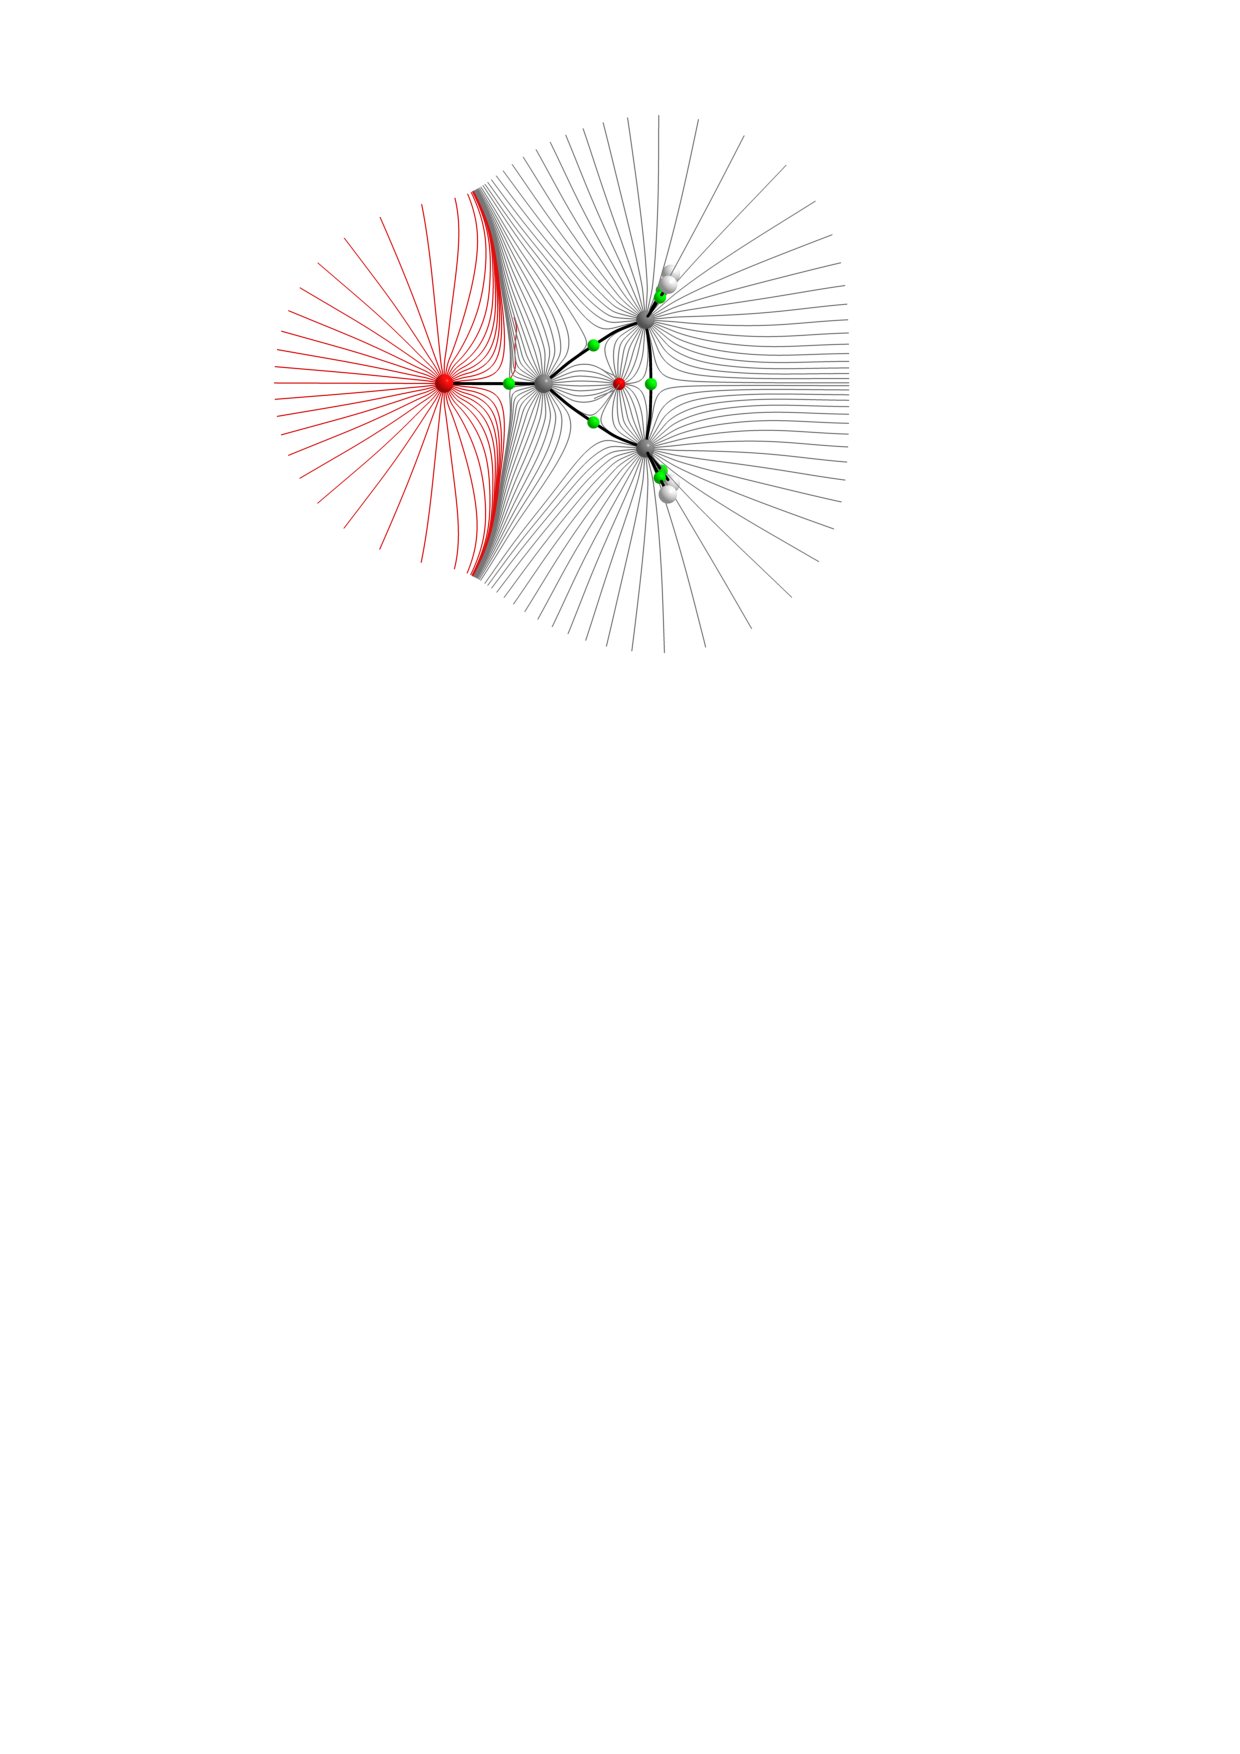
\includegraphics[width=0.4\textwidth]{3/img/flux}
  \caption{Flux lines $\nabla \rho(\mathbf{r})$ of the cyclopropanone molecule
  (C$_3$H$_4$O). These trajectories delimit regions that can be identified as
  atoms~\cite{todd}.}
\label{flux}
\end{figure}

As shown in Figure \ref{flux}, the borders of the space regions known as atoms
satisfy the zero condition flux \ref{cero_f} and in general, an analysis of
maximum and minimum electronic density can be done with the values in Table
\ref{PuntosCriticos}.

\subsection{Atom properties in molecules}

The regions $\Omega$ defined in QTAIM are identified as atoms in chemistry, and
it is provable that the postulates of quantum mechanics are fulfilled within
these atomic basins~\cite{bader}. Taking the zero flux condition, for an atom
inside a molecule, we come to a variational definition of the properties that
the subsystem has~\cite{Bieglerknig1982}.  Starting from the borders,
identified as interatomic surfaces, and the molecular structure, the molecular
properties are defined as the addition of all atomic properties:

\begin{equation}
  A = \sum_{\Omega}{a_{\Omega}},
\label{promoleculares}
\end{equation}

\noindent where $A$ is the molecular property and $a_{\Omega}$ is the same
property inside the basin $\Omega$. This is based on the atomic variational
principle, which states that if $\hat{A}$ is an operator equivalent to a sum of
monoelectronic operators, $\hat{A}=\sum\hat{a}$, the its expected value is
given by:
\begin{align}
  A(\Omega) \equiv \langle\widehat{A}\rangle_{\Omega} = \int_{\Omega}\int\cdots\int\int\cdots\int
  \left [ \frac{N}{2}\Psi_{el}^{\star}\hat{a}\Psi_{el} + (\hat{a}\Psi_{el})^{\star}\Psi_{el}\right ]
  d\omega_{1}\ldots d\omega_{N}d\mathbf{r_2}\ldots d\mathbf{r}_{N}d\mathbf{r}_{1} .
\end{align}

This implies that an atomic property is determined across the integration of an
associated operator density associated with that property,
\begin{align}
  \rho_{A}(\mathbf{r})=\frac{N}{2}\int\cdots\int\int\cdots\int[
  \Psi_{el}^{\star}\hat{a}\Psi_{el} + (\hat{a}\Psi_{el})^{\star}\Psi_{el}]
  d\omega_{1}d\omega_{2}\ldots d\omega_{N}d\mathbf{r_2}\ldots d\mathbf{r}_N ,
\end{align}
and
\begin{align}
  A(\Omega)=\int_{\Omega}\rho_{A}(\mathbf{r})\mathrm{d}\mathbf{r} .
\end{align}


\section{Interacting Quantum Atoms}\label{IQAtheory}

Interacting Quantum Atoms, \gls{IQA}, allows the electronic energy partition,
using mainly the density matrix~\cite{Blanco2005, mcweeny}. The first order
reduced matrix $\rho_1(\mathbf{r}_1;\mathbf{r}_1^{\prime})$ and the
pair-density $\rho_2(\mathbf{r}_1,\mathbf{r}_2)$ allow compute the
non-relativistic electronic energy within the Born-Oppenheimer approximation,
as was shown in Equation \ref{E_b-o},

\begin{align}
  E_{\mathrm{elec}} & = \frac{1}{2} \sum_{A \neq B} \frac{Z_A Z_B}{r_{AB}} 
    + \int \widehat{h} \rho_1(\mathbf{r}_1;\mathbf{r}_1^{\prime}) \mathrm{d} \mathbf{r}_1 
    + \frac{1}{2} \int \int \frac{\rho_2(\mathbf{r}_1,\mathbf{r}_2)}{r_{12}} 
    \mathrm{d} \mathbf{r}_1 \mathrm{d} \mathbf{r}_2, \label{base}\\
  E_{\mathrm{elec}} & = V_{\mathrm{nn}}
    + \langle \widehat{T} + \widehat{V}_{\mathrm{ne}} \rangle 
    + \langle \widehat{V}_{\mathrm{ee}} \rangle.
\end{align}

The monoelectronic energy is a sum of the kinetic energy and the
nucleus-electron attraction, \textit{i. e.}, $\widehat{h} = \widehat{T} +
\widehat{V}_{\mathrm{ne}}$, the other three terms $Z_X$,
$\widehat{V}_{\mathrm{nn}}$ and $\widehat{V}_{\mathrm{ee}}$ mean $i$)the atomic
number of $X$, $ii$) the internuclear repulsion and $iii$) the
electron-electron repulsion, respectively.

After a partition of the real space, as Bader proposed, and discussed in
previous sections, in where every space region is delimited by the zero flux
condition (Equation \ref{cero_f}) contains only one nucleus, \textit{i. e.},
the system has no non-nuclear attractor, then it is possible to rewrite the
Equation \ref{base} as:
%
\footnotesize
\begin{align} 
  E_{\mathrm{elec}}  &=  \frac{1}{2} \sum_{A \neq B} \frac{Z_A Z_B}{r_{AB}} 
    -\frac{1}{2} \int \nabla^2 \rho_1(\mathbf{r}_1;
    \mathbf{r}_1^{\prime}) \mathrm{d} \mathbf{r}_1
    -\sum_A  \int \frac{Z_A \rho(\mathbf{r}_1)}{r_{1A}} \mathrm{d} \mathbf{r}_1 
    +\frac{1}{2} \int \int \frac{\rho_2(\mathbf{r}_1,
    \mathbf{r}_2)}{r_{12}} \mathrm{d} \mathbf{r}_1
    \mathrm{d} \mathbf{r}_2 \nonumber \\
  &=  \frac{1}{2} \sum_{A \neq B} \frac{Z_A Z_B}{r_{AB}} 
    -\frac{1}{2} \sum_A  \int_A   \nabla^2 \rho_1(\mathbf{r}_1;
    \mathbf{r}_1^{\prime}) \mathrm{d} \mathbf{r}_1  
    -\sum_{AB} \int_B \frac{Z_A \rho(\mathbf{r}_1)}{r_{1A}} \mathrm{d} \mathbf{r}_1
    +\frac{1}{2} \sum_{AB} \int_A \int_B \frac{\rho_2(\mathbf{r}_1,
    \mathbf{r}_2)}{r_{12}} \mathrm{d} \mathbf{r}_1 \mathrm{d} \mathbf{r}_2 \nonumber \\
  &=  \frac{1}{2} \sum_{A \neq B} V_{\mathrm{nn}}^{AB}
    +\sum_A T_A + \sum_A V_{\mathrm{ne}}^{AA}
    +\sum_{A \neq B} V_{\mathrm{ne}}^{AB} + \sum_A V_{\mathrm{ee}}^{AA} 
    +\frac{1}{2} \sum_{A \neq B} V_{\mathrm{ee}}^{AB},
\end{align}
\normalsize

\noindent where the terms are given by:
%
\begin{align}
  V_{\mathrm{nn}}^{AB} &=  \frac{Z_A Z_B}{r_{AB}}, \label{VnnAB} \\
  T_A                  &= -\frac{1}{2} \int_A \nabla^2 \rho_1 (\mathbf{r}_1;\mathbf{r}_1^{\prime})
    \mathrm{d} \mathbf{r}_1, \label{cineticaMono} \\
  V_{\mathrm{ne}}^{AB} &= - Z_A \int_B \frac{\rho(\mathbf{r}_1)}{r_{1A}} \mathrm{d}
	  \mathbf{r}_1, \label{nucleoElecMono} \\
  V_{\mathrm{ee}}^{AB} &= \frac{2 - \delta_{AB}}{2} \int_A \int_B
	  \frac{\rho_2(\mathbf{r}_1,\mathbf{r}_2)}{r_{12}} \mathrm{d} \mathbf{r}_1
	  \mathrm{d} \mathbf{r}_2 \label{elecElec2Atoms}
\end{align}

The IQA partition divides electronic energy into two main components: $i$)
intra-atomic energy, which results from regrouping the terms:
%
\begin{equation} \label{eAtomo}
  E^A_{\mathrm{net}} = T^A + V_{\mathrm{ne}}^{AA} + V_{\mathrm{ee}}^{AA},
\end{equation}

\noindent and $ii$) the interaction between atom-pairs energy, which can be
obtained grouping the following terms:
\begin{equation} \label{e2Atomo}
  E^{AB}_{\mathrm{int}} = V_{\mathrm{nn}}^{AB} + V_{\mathrm{ne}}^{AB}
  + V_{\mathrm{ne}}^{BA} + V_{\mathrm{ee}}^{AB}
\end{equation}

The addition of these two contributions (Equations \ref{eAtomo} and
\ref{e2Atomo}), will result strictly in the total energy of the system,
%
\begin{equation} \label{eElec}
  E_{\mathrm{elec}} = 
    \sum_A E^A_{\mathrm{net}} + \frac{1}{2} \sum_{A \neq B} E_{\mathrm{int}}^{AB}
\end{equation}

In the Equation \ref{eElec} we can interpret $E_{\mathrm{elec}}$ as the
addition of intra- and inter-atomic contributions.  Additionally to the
partition of electronic energy that IQA proposes, the definition of the
internal energy of a fragment, or group of atoms, is of utmost importance for
the development of this work, since the definition of the inner energy of a
fragment, group of atoms, $\mathscr{G}$ is given by:

\begin{equation} \label{eG}
E^{\mathscr{G}}_{\mathrm{net}} = \sum_{A \in \mathscr{G}} E^A_{\mathrm{net}} 
	       +\frac{1}{2} \sum_{A\in \mathscr{G}}
		\mathop{\sum_{B \in \mathscr{G}}}_{B \neq A} E_{\mathrm{int}}^{AB}
\end{equation}

\noindent Then the interaction energy between two groups is defined as:

\begin{equation} \label{energiaGH}
  E^{\mathscr{GH}}_{\mathrm{int}} = \sum_{A \in \mathscr{G}} \sum_{B \in
    \mathscr{H}} E_{\mathrm{int}}^{AB}
\end{equation}

It is possible to have an expression for the energy analogous to the Equation
\ref{eElec}, since we are making groups of atoms, but in this case as a energy
function of the groups that form the system and the interaction energies
between them.
%
\begin{equation} \label{energiaGrupos}
  E_{\mathrm{elec}} = \sum_{\mathscr{G}} E^{\mathscr{G}}_{\mathrm{net}} 
  +\frac{1}{2} \sum_{\mathscr{G} \neq \mathscr{H}} E_{\mathrm{int}}^{\mathscr{GH}}
\end{equation}

%
The selection of atoms, and their interactions, which are in a fragment
$\mathscr{G}$ as the atoms which make a molecule inside a molecular cluster
give us a way to study the intermolecular interaction energy. And in that way,
it allows a direct comparison with the non-covalent interaction and the changes
that occur in the interactions when the fragment/molecule is in presence of
another molecule/environment.

\section{Electron Localization Function}\label{elftheory}

The Electron Localization Function (ELF) kernel, $\chi_{\sigma}$, can be
interpreted as a measure of the surplus of local kinetic energy due to the
Pauli Principle, in connection to the homogeneous electron gas kinetic energy
density~\cite{Savin1992}. The ELF, $\eta(\vec{r})$, is mapped through a
Lorentzian function \ref{lorentzian}, to a scale ranging from 0 (when
$\chi_{\sigma} \rightarrow \infty$) to 1 (when $\chi_{\sigma} \rightarrow 0$).

\begin{align}
  \mathbf{\eta(}\vec{r}) = \frac1{1+\chi_{\sigma}^{2}}
\label{lorentzian}
\end{align}

The gradient of this function, $\grad \eta$, is used to induce a topological
partition which divides the space into non-overlapping regions (basins). Their
properties can be determined by integrating the appropriate densities over
their associated volume. Hence, if one is interested in, for example, in lone
pairs populations, it suffices to integrate the electron density, $\rho$, over
the corresponding region associated to the lone pair
maximum~\cite{Munrriz2019}.

The energies of the different topological basins can be computed with
Interacting Quantum Atoms (IQA) energy decomposition scheme~\cite{Blanco2005}.
This approach provides a set of unique and rigorous energetic terms that
additively recover the exact energy of the system. Unlike many topological
analyses, this method is not only suitable for stationary points (\textit{e.g.}
equilibrium geometries), such as with virial related energy partitions, but
also for non-equilibrium geometries. This feature was crucial for evaluating
the energy terms along bond elongations in geometry scans. The energy terms are
calculated by partitioning the first- and second-order density matrices with
respect to the real space partitions, usually the QTAIM atomic basins, as in
the Equation \ref{eElec}, rewritten as:

\begin{align}
  E &=\sum_A (T_A + V^{AA}_{ee} + V_{en}^{AA}) + \sum_{A > B} (V_{en}^{AB} + V_{ne}^{AB} + V_{nn}^{AB} + V_{ee}^{AB}) \\\nonumber
    &=\sum_A E^A_{\mathrm{intra}} + \sum_{A>B} E_{\mathrm{inter}}^{AB}
\end{align}

In this thesis we will apply IQA to ELF partitions.  When considering bonding
basins (and valence in general) within the IQA partition, the nuclear terms
presented in the previous equations become null ($V_{en}^{BB}=0$,
$V_{nn}^{AB}=0$, $V_{en}^{AB}=0$). Therefore, for a bonding basin, which
interacts with the core basin that represents an atom $A$, the energy terms can
be expressed as shown in Equations \ref{intra_bond} and \ref{inter_bond},

\begin{align}
  E_{\mathrm{intra}}^{bond} = T^{bond} + V_{\mathrm{cou}}^{bond}
\label{intra_bond}
\end{align}

\begin{align}
  E_{\mathrm{inter}}^{A-bond} = V_{\mathrm{cou}}^{A-bond} + V_{\mathrm{XC}}^{A-bond}
\label{inter_bond}
\end{align}

This was the selected approach since we are interested in developing an energy
model accounting for interactions between electron pairs.  Its is possible to
calculate interactions between atoms and ``bonds'', as well as interactions
between two ``bonds'' and ``bonds'' with ``lone pairs''. For this purpose, the
original code was modified so as to perform integration tasks over ELF
basins~\cite{MartnPends2008}.

The IQA-ELF approach provides and accurate reference that can be used to
analyze the behaviour of the energy terms and to construct energy potentials
that take into account classical and non-classical terms. 

The original IQA implementation could only deal with a HF wavefunction.
However, recent developments provide support for DFT-derived
ones~\cite{Maxwell2016}.

\section{Non-Covalent Interactions}

Most chemical interactions are dominated by non-covalent interactions,
\textit{e. g.} folding of proteins, self-assembly of nanomaterials, or catalyst
and its substrate~\cite{Fenniri2001}. This class of interactions cover many
interactions, such as London dispersion, dipole-dipole interaction, hydrogen
bond, $\pi$-$\pi$ interactions, not leaving out repulsive
interactions~\cite{kollman1977noncovalent}.

The non-covalent interaction index is based on the density and its derivatives,
which since as mentioned in Section \ref{densidades}, has the advantage over
molecular orbital descriptors because it is an experimentally accessible scalar
field, also supported by the HK theorem~\cite{Hohenberg1964}.

Moreover, NCI simultaneously allows an analysis and a visualization of all
non-covalent interaction types as real-space surfaces. Thus, it is an important
tool to analyze chemical
systems~\cite{Julia_Contreras_G2011_1,ContrerasG2011_2}.

The mathematical core of NCI is the reduced density gradient $s(\rho)$,
(\gls{RDG}) it is a quantity from DFT used to describe how far away the system
lies from an homogeneous electron distribution.

\begin{align}
  s(\rho) = C_F^{-1} \frac{|\nabla\rho|}{\rho^{4/3}}
\label{s_def}
\end{align}

\noindent where $C_F^{-1}$ is the Fermi constant ($2(3\pi)^{1/3}$).

Using the above definition (Equation \ref{s_def}) we can exemplify an easy
case, a single atomic orbital $\psi = e^{-\alpha r}$, thus the density is $\rho
= e^{-2\alpha r}$ and the gradient is $\nabla\rho = -2\alpha\rho$, such that

\begin{align}
  s(\rho) = C_F^{-1}\frac{2\alpha\rho}{\rho^{4/3}} = \frac{2\alpha}{C_F}\rho^{-1/3}
\end{align}

The reduced density gradient assumes large values in the exponentially-decaying
density tails far from the nuclei. Small $s(\rho)$ values occur close to the
nuclei, due to the combination of large densities and small density gradients.
The lower bound on the reduced density gradient is zero~\cite{Narth2016}.

Analyzing $s(\rho)$ versus $\rho$ shows a new feature, one or more spikes in
low-density, low-gradient region are the signature of non-covalent
interactions.  This is the basis of NCI. When there is overlap between atomic
orbital, a peak appears on the $s(\rho)$ diagram, the points that form this
peak can identify the interaction when mapped the real space. Particularly, NCI
interaction index allows an analysis and a visualization of non-covalent
interactions types as real-space surface~\cite{Narth2016}.

The $s(\rho)$ isovalue determines which features will appear in the NCI plot.
Choosing large values would disclose atomic tails of the density. However, low
values might miss some of the interactions of interest~\cite{Lane2013}.

%\newpage

\section{Computational Details}\label{comp_details}

The geometries were taken from Force Field data bases. A single point
calculation was carried out in order to obtain the wavefunction for the
ELF/QTAIM analysis.  The single point was carried out at the
M06-2X/aug-cc-pVTZ~\cite{Zhao2006,Kendall1992,Woon1993} theory level, using the
suite of {\sc{Gaussian16}}~\cite{g16}. The choice of the functional and the
orbital basis was based on Jiménez Gravalos et al. work
\citenum{JimenezGravalos2019} in which it is shown the behaviour about the
\gls{HB} is well described for the water cluster with moderate computational
time.

Later on, using the electronic densities computed via DFT we proceeded to
analyse the topological properties of Electron Localization Function. Using the
TopMod, NCI plot and {\sc{Promelf}} programs for these purposes~\cite{topmod09,
Boto2020, promolden}. The visualization of our results was carried out with the
help of the {\sc{GausView}}~\cite{g16}, {\sc{VMD}}~\cite{HUMP96} and VESTA
\cite{vesta} codes.

The {\sc{Promelf}} program analyzes first order real space and momentum
molecular densities for a polyatomic molecule within basis set of GTO's
function, it can make a topological analysis for real space densities.  The
program was developed in 2002 by A. Martín Pendás at University of Oviedo.

In {\sc{Promelf}} code for the topology analysis all the 3D and 1D scalars, not
only their magnitudes, but also their first and second derivatives (gradients
and hessians) are computed analytically. This allows us to make automatic
topological analyses of them. A Morse consistency check is done on all
topologies, and paths connecting (3,-1) to (3,-3) points are traced and
studied~\cite{promolden}.

